\begin{savequote}[8cm]
  ``I have not failed. I've just found 10,000 ways that won't work.''
  \qauthor{Thomas Edison}
\end{savequote}
\makeatletter
\chapter{Methodology}

\section{Introduction}

Here we present several techniques used to extract dense 3D reconstruction from image/video data. In the first section we describe techniques in addition to Fourier volume registration. These include the recovery of translation, y-axis rotation and scale information as well as a technique for the recovery of a so called 7 degrees of freedom transform. \\

We also list notable speed-ups for volume registration which reduce the amount of processing by over a third. After this, a full 3D reconstruction technique based on the principles of phase correlation is presented. Then we also present two novel reconstruction data representations which may be used to efficiently represent and fuse 3D reconstructions. Lastly, different sensor inputs are discussed and some conclusions are given about the usefulness of this technique in the context of these sensors is presented.

\section{Fourier Volume Registration} 

\subsection{Recovery of Translation Values}

Given a volume $V_1$ and a spatially shifted version of it $V_2$, the offset along each axis, $(x,y,z)$ may be recovered if a suitable correlation between the two volumes can be found. \\

The measure of correlation between $V_1$ and $V_2$ can be found by shifting $V_1$ and $V_2$'s mean values to zero, then summing the element-wise multiplication of $V_1$ by $V_2$. Equation \ref{eqn:CorrelationEquation} computes this correlation measure.

\begin{equation} \label{eqn:CorrelationEquation}
\sum_{z=0}^{N}\sum_{y=0}^{N}\sum_{x=0}^{N}(V_1(x,y,z)-avg(V_1)) \times (V_2(x,y,z)-avg(V_2))
\end{equation}

Using this measurement, two volumes which are similar in signal shape (element-wise-value to location correspondence) will give a larger measure of correlation than two volumes with a differing signal shape. If the volumes are first normalized we can regard volume $x$ is more aligned with volume $y$ than with volume $z$ given $x$ correlated with $y$ gives a larger value than $x$ correlated with $z$. \\

Cross-correlation searches over a space of translation parameters and outputs the optimal translation to align two volumes. It is optimal in the sense of correlation measurement. This is used as a best guess in terms of the alignment of the two volumes. It can be thought of as the optimization of parameters $x,y,z$ in equation \ref{eqn:CrossCorrelationEquation}.

\begin{equation} \label{eqn:CrossCorrelationEquation}
CrossCorrelate(Transform(V_1, x,y,z), V_2)
\end{equation}

Since we typically do not know the range of translation values $x,y,z$ to optimize for, we take into account the range from $[0,N]$ where $N$ is the width/height/depth of the volume. This gives a complexity of $N^6$. This is too computationally complex for practical volume sizes. Therefore, we use the properties of the Fourier Transform to reduce computational complexity. \\
 
The 3D Fourier transform transforms a volume from the 3D spatial domain into the 3D frequency domain. The frequency domain is a complex valued volume made up of sinusoids where each value in the frequency domain represents the magnitude, phase and direction of a wave.  \\


WARNING: show picture of 3D volume fft\\

WARNING: show picture of 3D pc surface\\

Using the properties of the Frequency domain, we can efficiently recover the optimal alignment translation parameters using a function called $PhaseCorrelation$ (Eq. \ref{eqn:PC_basic}). This function takes two volumes as input and returns the best alignment translation between them in terms of maximizing correlation.
\begin{equation} \label{eqn:PC_basic}
(x, y, z) = PhaseCorrelation(V_x, V_y)
\end{equation}
The $PhaseCorrelation$ function first applies 3D FFTs to volumes, $V_1$ and $V_2$, converting them into the frequency domain, i.e. $F_{1_{x,y,z}} = FFT(V_1)$ and $F_{2_{x,y,z}} = FFT(V_2)$. Taking the normalised cross power spectrum using Eq. \ref{eqn:PHCOR_eq} based on these frequency domain volumes computes the frequency domain of a new volume called the phase correlation volume. \\


\begin{equation} \label{eqn:PHCOR_eq}
F_{3_{x,y,z}} = \frac{F_{1_{x,y,z}} \circ F_{2_{x,y,z}}^*}{ | F_{1_{x,y,z}} \circ F_{2_{x,y,z}}^* | }
\end{equation}

Here, $\circ$ is an element-wise multiplication and $|x|$ is the magnitude function. Taking the inverse FFT of the frequency domain of the phase correlation volume, $F_3$ gives the phase correlation volume itself, $V_3$ ($V_3 = FFT^{-1}(F_3)$). The location of the peak value in the phase correlation volume $V_3$, $(x_1, y_1, z_1)$ gives the shift between the $V_1$ and $V_2$. The phase correlation volume is typically noisy making the peak difficult to locate. Each in the phase correlation volume evaluates the correlation between $V_1$ (translated by the location of the peak) and $V_2$.


\subsection{Recovery of Y-Axis Rotation and Scale}

Using the phase correlation procedure along with some spatial transformation functions allows the computation of a single axis of rotation (out of 3) along with the scale difference between two volumes. If $V_1$ and $V_2$ are translated, rotated and scaled versions of the same volume, such that they are related by some translation $(t_x, t_y, t_z)$, y-axis rotation $\theta$, and scale $\varphi$.\\


WARNING: show picture of log-spherical transform\\

Here we describe how to compute the rotation and scale parameters, further action is required to recover translation. The first step, given two volumes $V_1$ and $V_2$ of size $N^3$ is to apply a Hanning windowing function (Eq. \ref{eqn:Hann}). This function assists in filtering the volumes prior to a discrete Fourier transform being applied to them. Since the discrete Fourier transform relies on a continuous signal (volume) and this cannot be used in the calculation, by reducing the signal strength near the volume borders, we can improve the accuracy of the discrete Fourier transform.
\begin{equation} \label{eqn:Hann}
\scriptstyle
HW_{x,y,z} = \frac{1}{2}\left(
1 - cos \left(
\frac{2\pi
\left(
\sqrt{\left(\frac{N}{2}\right)^3} -
\sqrt{
\left(x-\frac{N}{2}\right)^2 + \left(y-\frac{N}{2}\right)^2 + \left(z-\frac{N}{2}\right)^2
}
\right)
}
{2\sqrt{\left(\frac{N}{2}\right)^3} - 1}
\right)
\right)
\end{equation}
The rotation and scale factors can only be recovered if translation information is removed from the two volumes. Therefore we take the magnitude of the FFT of the volumes, $M_1 = |FFT(V_1)|$, $M_2 = |FFT(V_2)|$. Since the magnitude values do not contain phase information they do not, by nature, contain location information of the volume (translation information). The zero-frequency of both $M_1$ and $M_2$ is next shifted to the center of the volume and the log of the result is taken $M'_1 = Log(M_1)$, $M'_2 = Log(M_2)$. Like in phase correlation the log function spreads out the contribution of the frequencies so that high frequencies contribute as much as lower frequencies which have larger magnitudes. A log-spherical transform is then used to turn rotation and scaling into translation for both $M'_1$ and $M'_2$. Eq. \ref{eqn:Log_Spherical} shows the corresponding log-spherical space coordinate $(X_{log-spherical}, Y_{log-spherical}, Z_{log-spherical})$ for a given $(x,y,z)$ euclidean space coordinate.
\begin{equation} \label{eqn:Log_Spherical}
\begin{split}
X_{log-spherical} & = \frac{atan\left(
\left(\frac{x-\frac{N}{2}}{\sqrt{x^2+y^2+z^2}}\right)
\left(\frac{y-\frac{N}{2}}{\sqrt{x^2+y^2+z^2}}\right)^{-1}
\right)N}{360}\\
Y_{log-spherical} & = \frac{acos\left(
\frac{y}{\sqrt{x^2+y^2+z^2}}
\right)N}
{180} \\
Z_{log-spherical} & =\frac{log\left(\sqrt{x^2+y^2+z^2}\right)N}{log\left( \frac{N}{2.56} \right)} \\
\end{split}
\end{equation}
The log-spherical transforms of $M'_1$ and $M'_2$ are then phase correlated to find the shift between them, $(x_{M'},y_{M'},z_{M'}) = PhaseCorrelation(M'_1, M'_2)$. The rotation $\theta$ and scale $\varphi$ factors between $V_1$ and $V_2$ can then be found from the shift parameters using Eq. \ref{eqn:ROTATIONSCALEFROMXM} . 
\begin{equation} \label{eqn:ROTATIONSCALEFROMXM}
\begin{split}
\theta & = \frac{-360x_{M'}}{N}\\
\varphi & = e^{
-\left(
2.56^{-1}N
\right)z_{M'}N^{-1}
}
\end{split}
\end{equation}
Using $\theta$ and $\varphi$, $V_1$ can now be inverse transformed (using $(\frac{N}{2}, \frac{N}{2}, \frac{N}{2})$ as the origin). This aligns $V_1$ and $V_2$ with respect to scale and y-axis rotation. The translation parameters $(t_x, t_y, t_z)$ can then be found using phase correlation as given in Eq. \ref{eqn:FINALTRANS}.
\begin{equation} \label{eqn:FINALTRANS}
(t_x, t_y, t_z) = PhaseCorrelation(scale(rotate(V_1,\theta),\varphi), V_2)
\end{equation}
The complete function to recover translation, rotation and scaling, combining equations \ref{eqn:PHCOR_eq}-\ref{eqn:FINALTRANS} as is denoted in \ref{algorithm:PCSLAM} is \ref{eqn:FULLPC}.
\begin{equation} \label{eqn:FULLPC}
(\theta, \varphi, t_x, t_y, t_z) = PhaseCorrelation_{\theta \varphi t_x t_y t_z}(V_m, V_n)
\end{equation}

\subsection{Full Recovery of 3D Rotation}

\label{FullRecovery3DSection}

In order to recover full 3D rotation (as well as scale and translation) the model must first be aligned by some common axis. PCA or Principals Component Analysis is a well known technique for recovering the primary axes of an N-dimensional signal. In this case, we can use the most accurate axis (the eigen-vector with the largest corresponding eigen-value) to align two volumes, then y-axis rotation, scale and translation values can be recovered by the described FFT based volume registration method. \\

WARNING: SHOW picture of this PCA procedure

PCA is a capable registration technique on its own, but when faced with non-overlapping, missing or noisy data it typically fails on its own. The technique of alignment is discussed in the following sections. \\

Given a 3-dimensional signal $A$ of length $N$, the co-variance of the signals between two of the dimensions ($x$ and $y$) is given as a function in equation \ref{eqn:Covariance3DSignal}.

\begin{equation} \label{eqn:Covariance3DSignal}
Cov(A_x,A_y) = \sum_{i=0}^{N}(A_{x_i} - A_{x_{mean}})(A_{y_i} - A_{y_{mean}})
\end{equation}

Here, $A_{x_{mean}}$ and $A_{y_{mean}}$ are the mean values of these x and y dimensions of $A$. 

Using the voxel locations of volume $A$ we can generate the covariance matrix \ref{eqn:CovarMatrix}. This matrix describes the how each coordinate changes with respect to each other.

\begin{equation} \label{eqn:CovarMatrix}
\left[
\begin{array}{ccc}
Cov(A_x, B_x) & Cov(A_x, A_y) & Cov(A_x, A_z) \\
Cov(A_y, B_x) & Cov(A_y, A_y) & Cov(A_y, A_z) \\
Cov(A_z, B_x) & Cov(A_z, A_y) & Cov(A_z, A_z) \\
\end{array}
\right]
\end{equation}

The 3 eigen-vectors of the covariance matrix describe the primary axis of the signal $A$ and the 3 corresponding eigen-values describe the strength of these axes. The eigen-vector/axis with the largest corresponding eigen-value is the principal component. The principal component is used to align data to a common axis. Here we define the principal axis (component) of a 3D signal $A$ as $A_{pa}$. \\

Given a 3D volume $V$, with a computed principal axis $V_{pa}$ and mean $V_{mean_location}$, we can construct a matrix to normalize the 3D data in terms of the principal axis.

Given $V_{pa}$ a vector pointing along the principal axis of $V$, we compute the forward vector as 


\begin{equation} \label{eqn:fwdVector}
Fwd = \left(\left[
\begin{array}{c}
V_{pa_{x}}\\
V_{pa_{y}}\\
V_{pa_{z}}\\
\end{array}
\right] \times \left(\left[
\begin{array}{c}
1\\
0\\
0\\
\end{array}
\right] \times \left[
\begin{array}{c}
V_{pa_{x}}\\
V_{pa_{y}}\\
V_{pa_{z}}\\
\end{array}
\right]\right)\right) \times \left[
\begin{array}{c}
V_{pa_{x}}\\
V_{pa_{y}}\\
V_{pa_{z}}\\
\end{array}
\right]
\end{equation}

Here, $\times$ is the cross-product of the vectors. The right pointing vector is computed as orthogonal to the forward vector and the common vertical axis $V_{pa}$,


\begin{equation} \label{eqn:fwdVector}
Rgt = \left[
\begin{array}{c}
V_{pa_{x}}\\
V_{pa_{y}}\\
V_{pa_{z}}\\
\end{array}
\right] \times \left[
\begin{array}{c}
Fwd_x\\
Fwd_y\\
Fwd_z\\
\end{array}
\right]
\end{equation}

Then the volume can be normalized to an axis based on the input data. This is done using a matrix which transforms the data to the origin, then corrects the vector $V_{pa}$ to be the new up axis, then transforms back. The matrix in equation \ref{eqn:CorrectUpMat} computes this,


\begin{equation} \label{eqn:CorrectUpMat}
CorrectMat(V) = \left[
\begin{array}{cccc}
1 & 0 & 0 & V_{mean_x} \\
0 & 1 & 0 & V_{mean_y} \\
0 & 0 & 1 & V_{mean_z} \\
0 & 0 & 0 & 1 \\
\end{array}
\right] \left[
\begin{array}{cccc}
Rgt_x & Rgt_y & Rgt_z & 0 \\
V_{pa_x} & V_{pa_y} & V_{pa_z} & 0 \\
Fwd_x & Fwd_y & Fwd_z & 0 \\
0 & 0 & 0 & 1 \\
\end{array}
\right] \left[
\begin{array}{cccc}
1 & 0 & 0 & -V_{mean_x} \\
0 & 1 & 0 & -V_{mean_y} \\
0 & 0 & 1 & -V_{mean_z} \\
0 & 0 & 0 & 1 \\
\end{array}
\right]
\end{equation}


To recover a matrix for full 3D rotation, scale and translation for given volumes $Volume_A$ and $Volume_B$, we first compute the correction matrices using PCA and the technique described above for both $Volume_A$ and $Volume_B$ as $C_A = CorrectMat(Volume_A)$ and $C_B = CorrectMat(Volume_B)$. The transformation matrix relating $Transform(Volume_A, C_A)$ and $Transform(Volume_B, C_B)$ is computed as $RST$. The final transform then relating $Volume_A$ to $Volume_B$ is computed as,

\begin{equation} \label{eqn:FullRSTTransform}
R_{x,y,z}ST Matrix = C_{B}^{-1} \times RST \times C_A
\end{equation}

This technique is capable of extending Fourier registration to take into account full 3D rotation. The technique simply requires a single iteration over the data to compute the principal components then a rotation-scale-translation phase correlation technique is used to compute the scale, translation and y-axis rotation. 

WARNING: show an example of this working

\subsection{Filtering Techniques}

\subsection{Fast Fourier Volume Registration}

3D phase correlation is CPU and GPU intensive, so in order to reduce complexity we tried to minimize processing in areas which require the most computation time. In out Fourier based volume registration method defined in the previous section, this occurs in the two 3D phase correlations which need to be computed. We describe the method of reduction here; a block diagram for this technique is given in figure \ref{fig:PIPELINE3} WARNING:Given a picture for the sped up version too!. We refer to this method as fast volume registration (FVR) in reference to general volume registration (VR). The speedup begins by computing the 3D DFT of both input volumes and taking the magnitude of these. Rather than directly performing a 3D log-spherical transform and a 3D phase correlation operation on these volumes, we use a novel transform we call a spherical-map transform (details in \ref{SMTransform}).\\

\begin{figure*}[t]
\centering
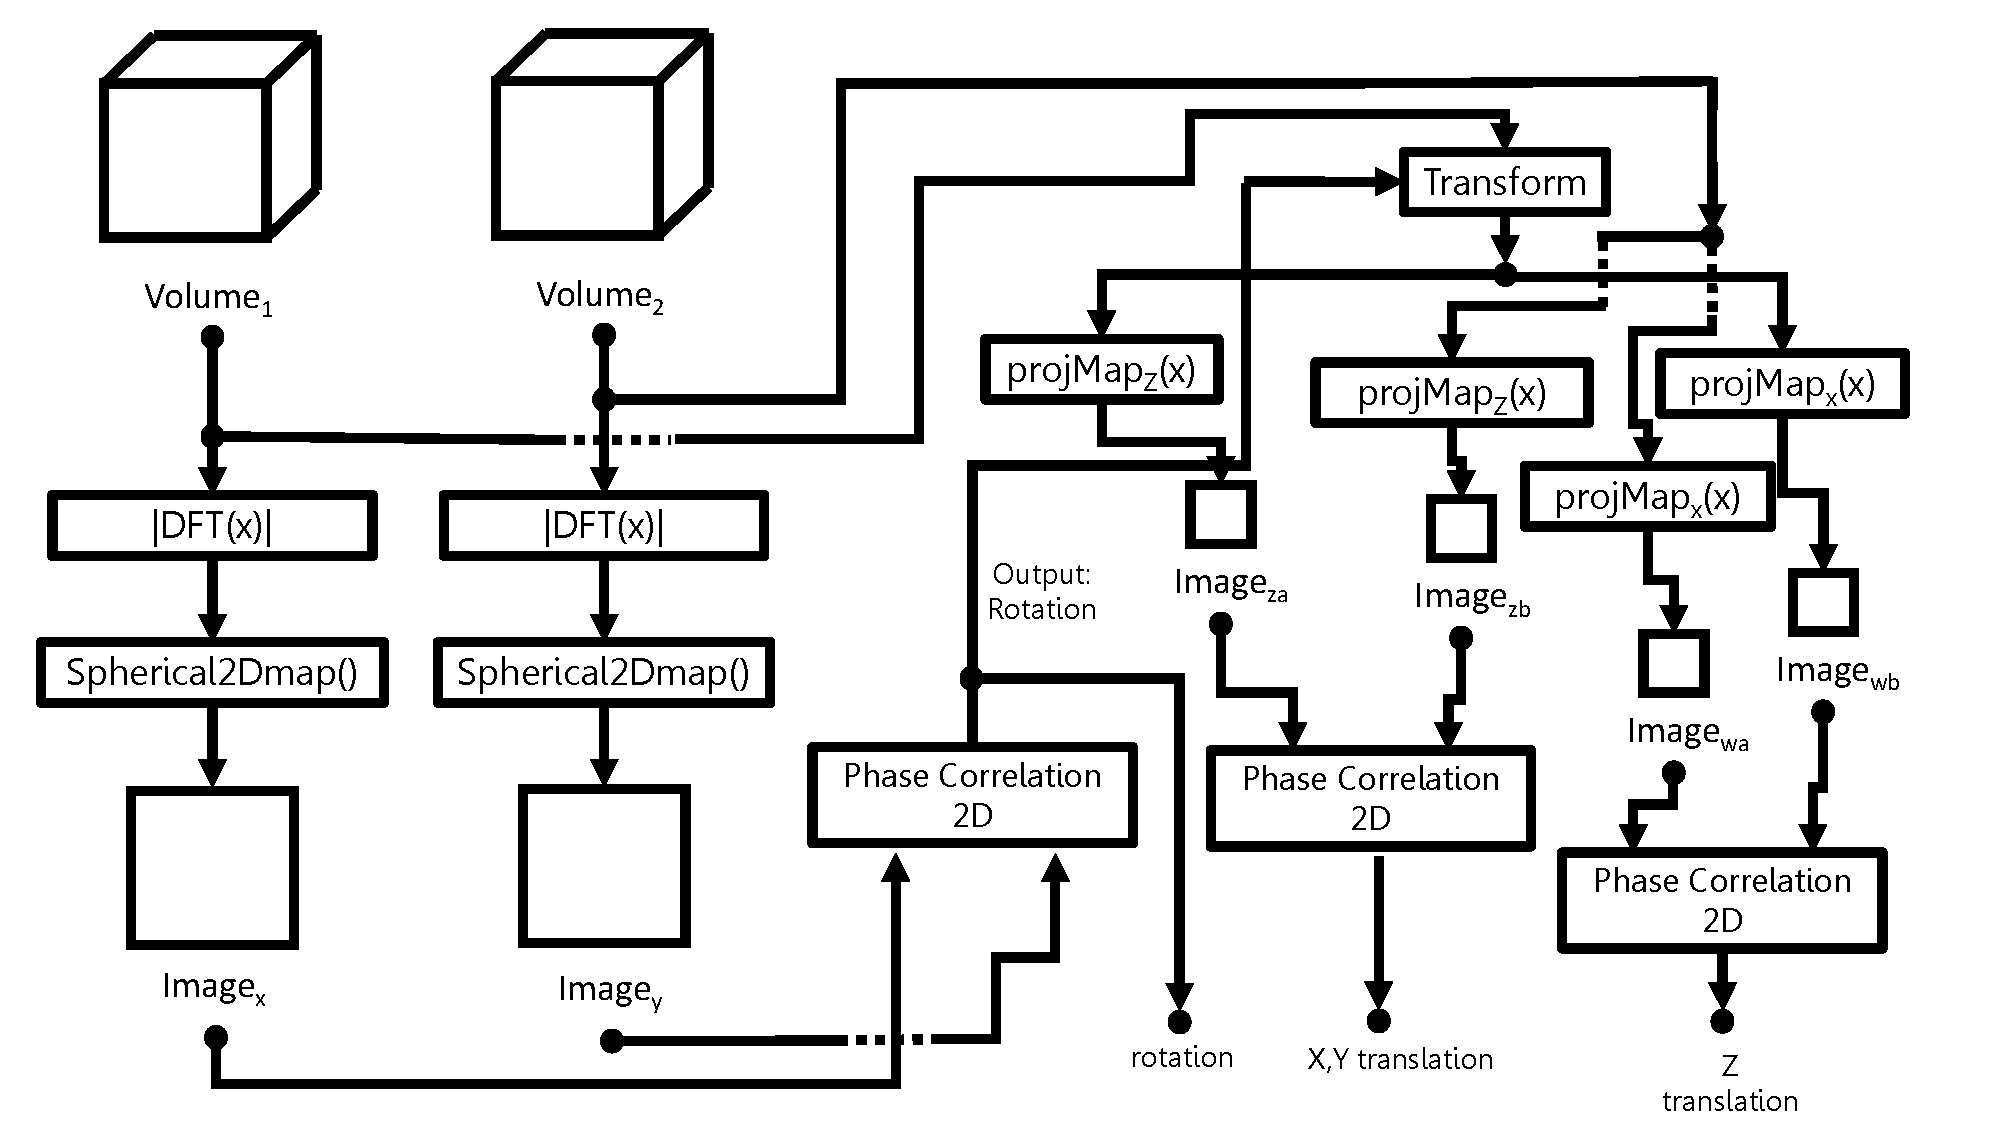
\includegraphics[width=6.0in]{images/ch2/pipeline3}
\caption{System Diagram for Fast Volume Registration}
\label{fig:PIPELINE3}
\end{figure*}

This transform converts rotation into translation whilst simultaneously unfolding the 3D space down to 2-dimensions. After this, a 2D phase correlation that requires significantly less processing compared with the 3D counterpart is used to compute the rotation. Next, having obtained the rotation parameter, the rotation is eliminated from the transformation by rotating the first volume by this parameter. The two volumes are then passed through two orthogonal projection mapping functions. This also converts the volumes to 2D space. We use two transforms for both volumes, one projection along the x-axis, another along the z-axis. Once the x-axis projections of both volumes are complete, we can do another 2D phase correlation to give us the z-translation. The 2D phase correlation of the z-axis projections gives us the x and y axis translations separating the original volumes. The final output of this method gives the rotation and translational shifts between the input volumes. The projections add little complexity to the overall algorithm and since 2D phase correlation operations are used in place of 3D ones, much computation time is reduced.

\subsection{Spherical-map transform}
\label{SMTransform}
The spherical map transform both reduces the 3D volume to a 2D image, and any rotation about the y-axis becomes x-axis translation in the output image. An example of the bunny model and the spherical-map transform of this model is given in figure \ref{fig:smtExample}, the mathematics are defined in equations \ref{eqn:invLPFuncs} and \ref{eqn:smtUpdate}. Given a coordinate in 2D Cartesian space x,y, we compute the ray $[Ray_x Ray_y Ray_z]^T$ from the volume center and sum up the voxel values along the ray (equation \ref{eqn:smtUpdate}). \\


\begin{equation} \label{eqn:invLPFuncs}
\begin{split}
Ray_x(x,y) & = cos\left(\frac{360x}{N}\right)sin\left(\frac{180y}{N}\right)  + \frac{N}{2} \\
Ray_y(y) & = cos\left(\frac{180y}{N}\right) + \frac{N}{2} \\
Ray_z(x,y) & = 	sin\left(\frac{360x}{N}\right)sin\left(\frac{180y}{N}\right) + \frac{N}{2}
\end{split}
\end{equation}

\begin{equation} \label{eqn:smtUpdate}
Im_{x,y} = \sum_{r=1}^{(2^{-1}N)^{1.5}}{Vol(Ray_x(x,y)r, Ray_y(y)r, Ray_z(x,y)r)} 
\end{equation}

This process essentially sums up the values along a given ray defined by scaling spherical coordinates and adding up the values intersecting the ray. The resulting image, maps 3D y-axis rotation to 2D x-axis translation.  \\

\begin{figure*}[t] 
        \centering
        \begin{subfigure}[b]{4.2in}
                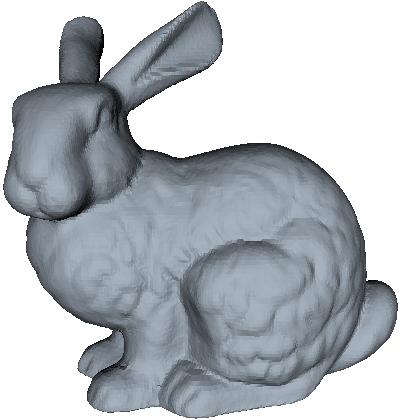
\includegraphics[width=4.2in]{images/ch2/bunny}
                \caption{original}
                \label{fig:bunnyOrig}
        \end{subfigure}
        \begin{subfigure}[b]{4.2in}
                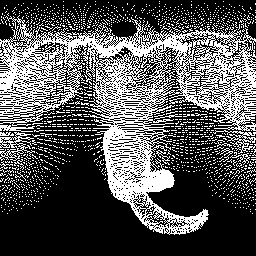
\includegraphics[width=4.2in]{images/ch2/spherical2DMap}
                \caption{transform}
                \label{fig:bunnySPTed}
        \end{subfigure}%
        \caption{The Spherical Map Transform.}
       \label{fig:smtExample}
\end{figure*}


\subsection{Projection-map transform}

The projection map transform is similar to an orthogonal projection of the volume along some given axis. For the projection map transform, given an output image $Im_a$ and an input volume $Vol_a$, each pixel in $Im_a$ is defined mathematically as the summation of values along a particular axis given the image coordinates. The x-axis transform and the z-axis transform are defined in equations \ref{eqn:xPMT} and \ref{eqn:zPMT} respectively. \\

WARNING: add in a picture here

\begin{equation} \label{eqn:xPMT}
Im(z,y) = \sum_{x=0}^{N}{Vol_a(x,y,z)}
\end{equation}

\begin{equation} \label{eqn:zPMT}
Im(x,y) = \sum_{z=0}^{N}{Vol_a(x,y,z)}
\end{equation}

The process defined by equation \ref{eqn:xPMT} maps 3D z-axis translation to 2D x-axis translation, whilst equation \ref{eqn:zPMT} maps 3D x-axis and y-axis translation into 2D x-axis and y-axis translation.


To assess the performance of our method, the size of the volumes being registered is defined as $N^3$ whilst each frame is sampled at a resolution of $W$ $\times$ $H$. The projection process requires $12WH$ operations whilst re-sampling the point cloud requires $2WH$ operations. The Volume Registration process, $VolumeRegister{\theta \varphi t_x t_y t_z}(V_1, V_2)$ consists of 2 $\times$ Hanning windowing processes, 2 $\times$ 3D FFTs, 2 $\times$ volume-logs, 2 $\times$ log-spherical transforms, 2 $\times$ phase correlation processes and 1 $\times$ linear transformation and peak finding. 

The Hanning windowing function requires 26 operations. The 3D FFT has complexity of $3N^3\log{N}$, the log and log-spherical transform functions require 3 and 58 operations per voxel respectively. Multiplying two frequency spectra together and transforming a volume requires 15 and 30 operations per voxel respectively. Finding the peak value requires $2N^3$ operations. The complexity in terms of number of operations for the phase correlation process is given in Eq. \ref{eqn:PCFULLPERFORMANCE} This process requires 2 $\times$ 3D FFTs, 1 $\times$ frequency spectra multiplication, and 1 $\times$ peak finding operation. 
\begin{equation} \label{eqn:PCFULLPERFORMANCE}
6N^3\log{N} + 2N^3 + 15
\end{equation}
The total complexity can then be found by taking into account the projection and re-sampling totals as well as the total for $VolumeRegister{\theta \varphi t_x t_y t_z}(V_1, V_2)$. Tallying the number of operations for each process and multiplying them by number of times the process is performed gives us the number of operations as a function of $W$, $H$ and $N$ in Eq. \ref{eqn:FULLPERFORMANCE}.
\begin{equation} \label{eqn:FULLPERFORMANCE}
6N^3 + 28WH + 18(N^3\log{N}) + 230
\end{equation}



To compare performance of the generic volume registration method with the speed up, we use the complexity defined in equation \ref{eqn:FULLPERFORMANCE}. Here, we ignore the cost of projecting the depth map. The 3D DFT has complexity $3N^3log(N)$. This is the first step (see figure \ref{fig:PIPELINE3}), the next is the spherical-map transform which is complexity $45N^3$. If processed on the GPU the performance becomes 45 operations per voxel assuming that one voxel is assigned to one unit of processing. A 3D transform is 30 operations per voxel, 2D phase correlation requires 15 operations to multiply the frequency spectra and $2N^2log(N)$ operations to do the 2D FFT. Finally a projection map transform requires 1 operation per voxel. \\

In total, the proposed method requires $2 \times$ 3D FFTs, $2 \times$ spherical-map transforms, $1 \times$ 3D geometrical transformation, $3 \times$ 2D phase correlations and $4 \times$ projection map transforms. The total complexity is added up for all of these functions and given in equation \ref{eqn:FULLPERF2}. \\

\begin{equation} \label{eqn:FULLPERF2}
6log(N)\times (N^3 + N^2) + 169
\end{equation}

Figure \ref{fig:perfComp} provides a visualization of the performance improvement which the proposed method achieves over the original Fourier volume registration approach. It is clear that the proposed method is around 3 times faster
than the original Fourier based volume registration approach. This is due to the reduction in the amount of data to process afforded by the novel spherical-map transform and orthogonal projection methods.

\begin{figure}[t]
\centering
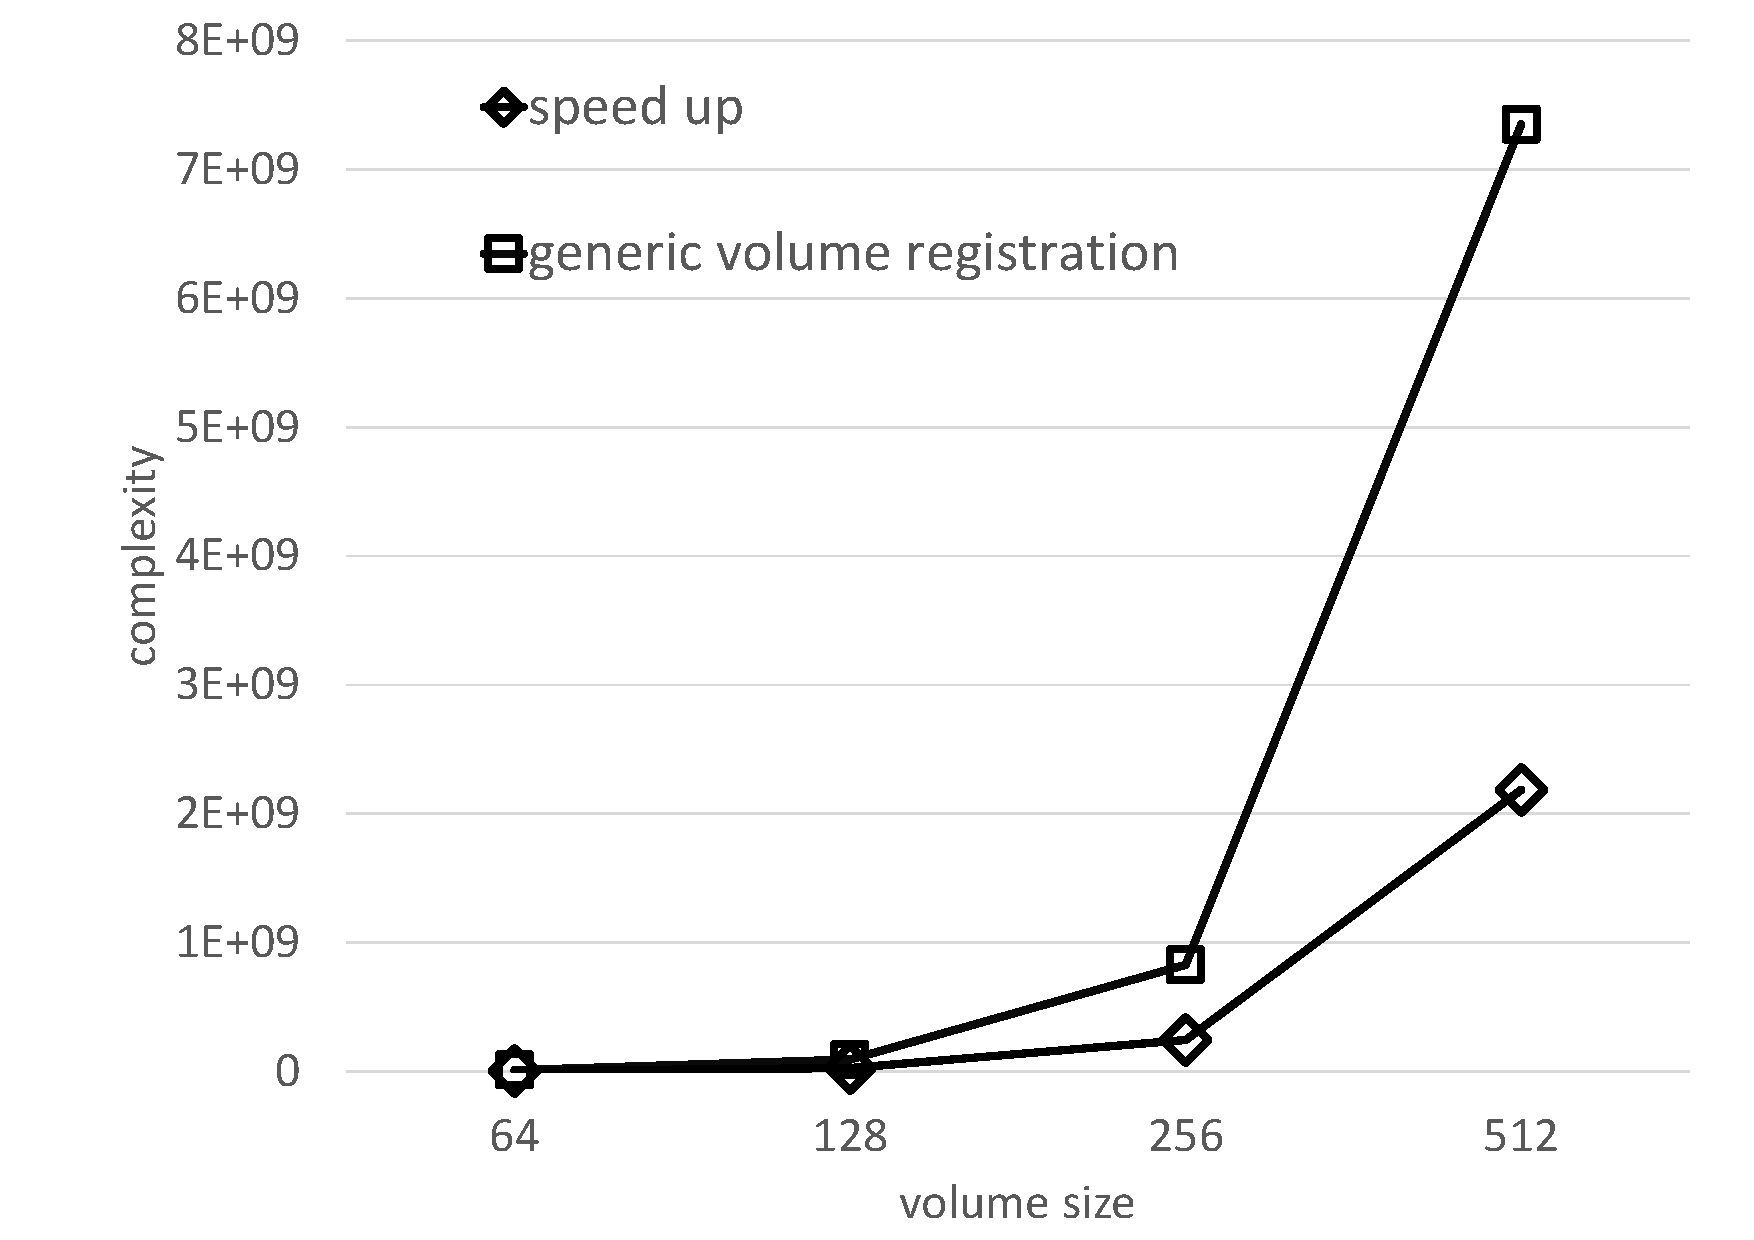
\includegraphics[width=4.0in]{images/ch2/perfcomp}
\caption{Comparison of performance between volume registration and the proposed speed up for different volume sizes.}
\label{fig:perfComp}
\end{figure}



\section{Fourier Volume Registration based 3D Reconstruction}


In this section we describe the general technique of recovering pose estimation via Fourier volume registration techniques. Several methods may be used and each has its own advantages and disadvantages and suitability depends on pose restriction, camera accuracy, noise levels and input data. 


\subsection{A Volume Registration based 3D Reconstruction Pipeline}

\label{METHOD_SECLL}
The proposed 3D reconstruction method consists of various steps. First each frame $f_i$ that is captured, consisting of a colour and depth image pair is projected into 3D space, forming colour point cloud $points_i$ and re-sampled into a volume $V_i$. Then, the transform parameters between pairs of volumes $V_i$ and $V_{i+1}$ are estimated using $VolumeRegister_{\theta \varphi t_x t_y t_z}$ shortened to $VR_{\theta \varphi t_x t_y t_z}$. These parameters are used to update transformation matrix $M$. The points corresponding to $f_2$ ($points_1$) are then transformed using the updated $M$ matrix and added to the cumulative $PointCloud$ database. Two lists, $Cameras$ and $Poses$, are also updated to track camera pose and location per frame. This basic procedure is given in listings \ref{algorithm:PCSLAM} and elaborated upon in subsequent subsections.
\begin{figure}
\begin{lstlisting}[language=c++,caption=Phase Correlation Based SLAM Algorithm,label=algorithm:PCSLAM,mathescape,basicstyle=\ttfamily]
$f_1$ = ReadFrame();
$PointCloud$ = project($f_1$);
$M$ = IdentityMatrix();
$Camera$ = $[0, 0, 0]^T$;
$Pose$ = $[0, 0, 1]^T$;
$Cameras$ = $\left[Camera\right]$, $Poses$ = $\left[Pose\right]$;
while(more frames){
	$f_2$ = ReadFrame();
	$points_1$ = project($f_2$);
	$points_2$ = project($f_1$);
	$V_1$ = ResampleVolume($points_1$);
	$V_2$ = ResampleVolume($points_2$);
	$(\theta, \varphi, t_x, t_y, t_z) = VR_{\theta \varphi t_x t_y t_z}(V_1, V_2)$;
	$M = M \times$TransformMat($(\theta, \varphi, t_x, t_y, t_z)$);
	$points_1$ = Transform($points_1$, $M$);
	$PointCloud$ = $PointCloud \cup points_1$;
	$Camera$ = $M^{-1} \times Camera$;
	$Pose$ = $M^{-1} \times Pose$;
	$Cameras.add(Camera)$;
	$Poses.add\left(\frac{Pose-Camera}{|Pose-Camera|}\right)$;
	$f_1$ = $f_2$;
}
\end{lstlisting}
\end{figure}


The input to our method is a color and depth image pair, $f(u,v)$ and $g(u,v)$ obtained using an Asus Xtion PRO LIVE sensor at a resolution of $640 \times 480$. Each pixel is projected into 3D space using $X_{u,v} = \frac{(u - c_x)Z_{u,v}}{f}$, $Y_{u,v} = \frac{(v - c_y)Z_{u,v}}{f}$ and $Z_{u,v}$ = $g(u,v)$. 
Here, $[c_x c_y]^T$ represent the center of the image whilst $f$ represents the focal length, defined as $525.0$. The point clouds generated by projecting these images are then quantized into image volumes. Results reported in this paper were obtained using volumes of $384^3$ voxels in size.

\begin{figure*}[t]
\centering
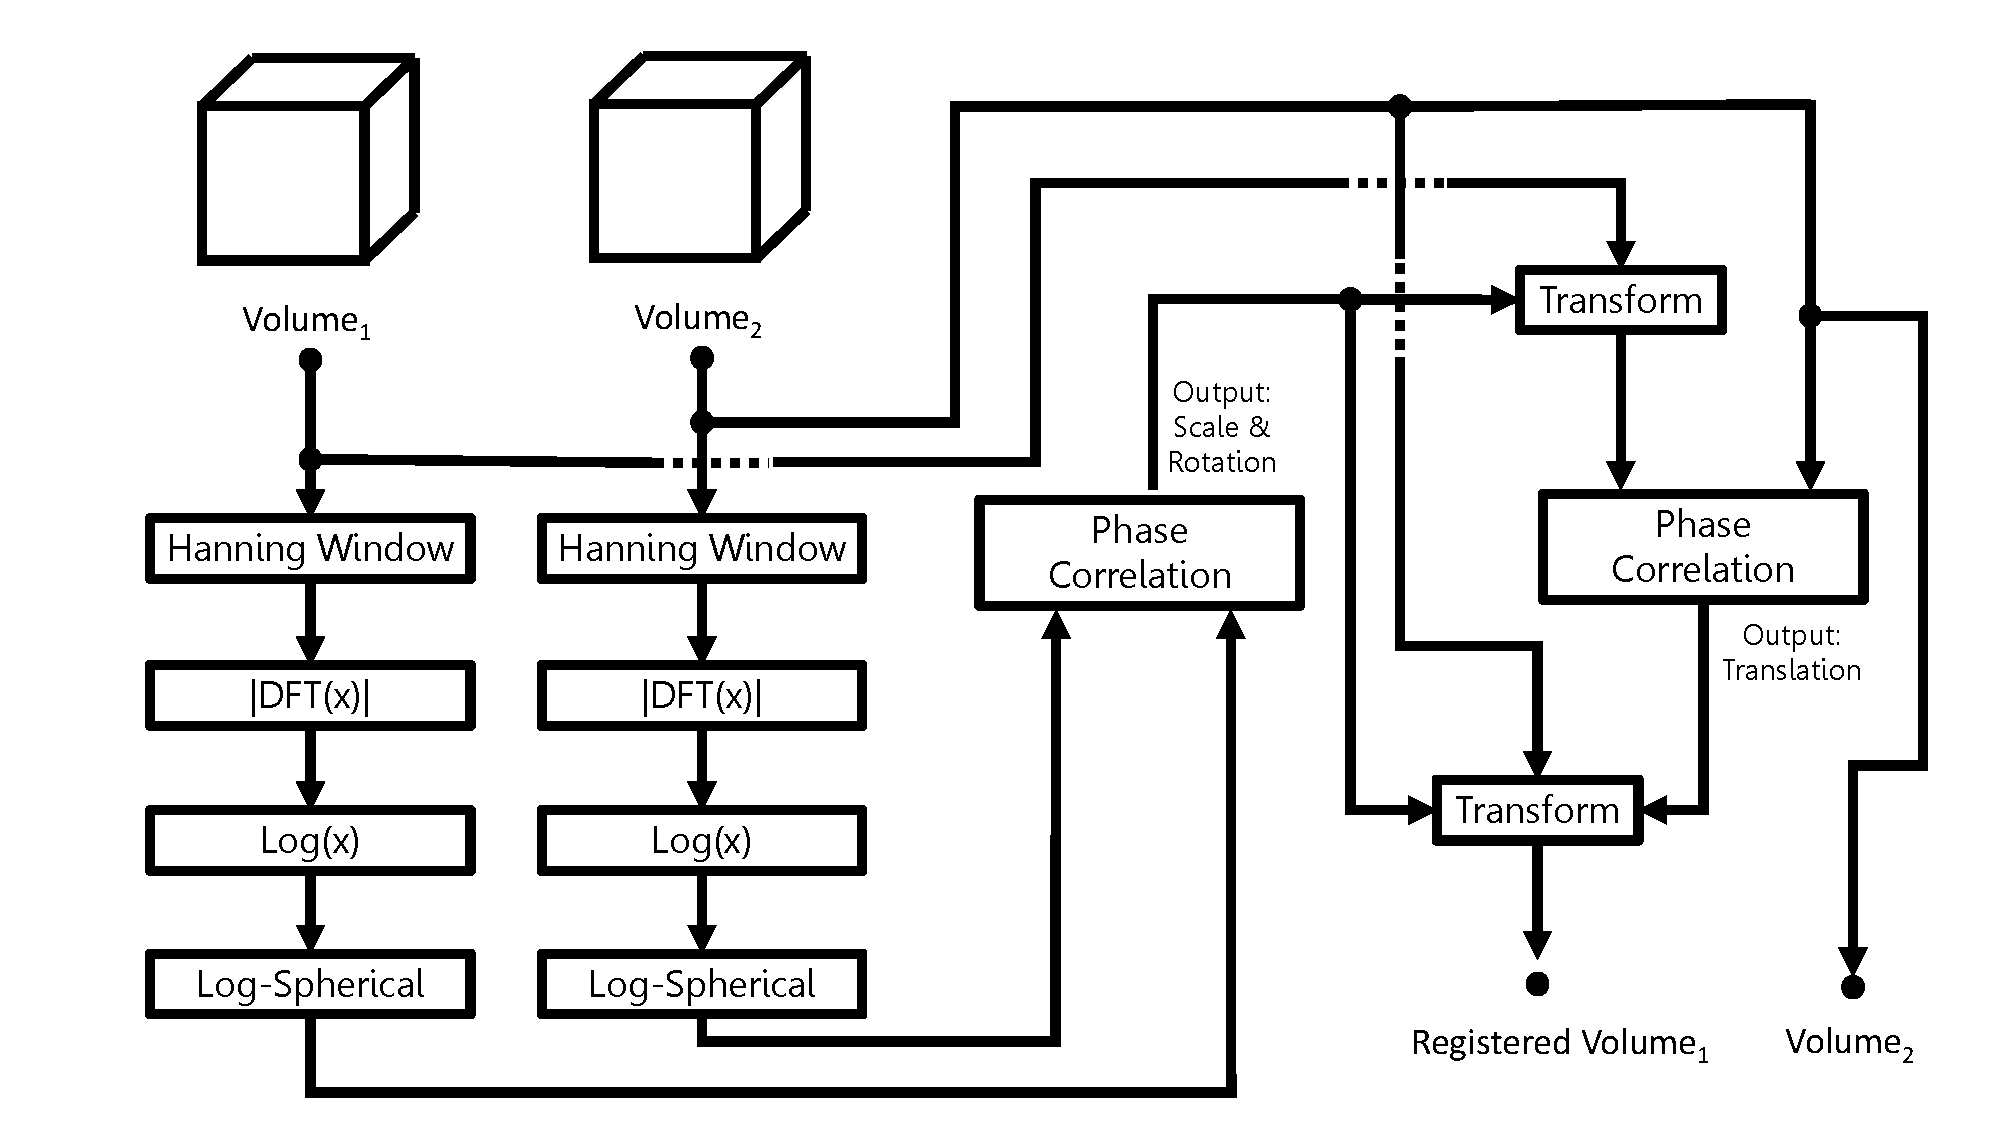
\includegraphics[width=6.0in]{images/ch2/pipeline2}
\caption{System Diagram for Registration Process}
\label{fig:PIPELINE}
\end{figure*}


\subsection{Error metrics}

In order to evaluate the accuracy of volume registration we use several error metrics including: Hausdorff error, mean squared error and the percentage of matched voxels. We describe mathematically those techniques here. All measurements are based on a simple function which computes the nearest neighbour for a given 3D point or voxel given a volume (or collection of 3D points). We define such a function, named nearest-neighbour in equation \ref{eqn:NN}.

\begin{equation} \label{eqn:NN}
NN(p, V) =  \{ q \in V | (Dist(q, p) < Dist(k, p))  \forall k \in V \}
\end{equation}

This function retrieves the closest corresponding point given a query point $p$ and a volume or point cloud of points, $V$. This function can be used to provide omni-directional error functions based on Hausdorff, mean squared and percentage accuracy error metrics.

Here some one-way error functions are described. The one was Hausdorff error is defined in \ref{eqn:HDOW} 

\begin{equation} \label{eqn:HDOW}
\sum_{k=0}^{N} Dist(P_k, NN(P_k, Q))
\end{equation}

\subsection{Reconstruction Integration}

Using the techniques of registration described in the above sections, there are several techniques which may be used to integrate these registered data. In most experiments we use the volume integration to combine the registered data in a single global model. We also propose several techniques for data representation and evaluate their abilities (see section \ref{sec:3DDataRepresentations}). As for the typical volume integration used, we create volumes with dimensions of $512\times 512\times 512$, although larger sizes may be used for increased accuracy. Once a frame is registered, it is projected into the volume. \\

This projection follows the following formula


\begin{equation} \label{eqn:volIntegration}
\begin{split}
x^{1} & = floor((x - frameCenter_x) \times scalar + volumeCenter_x) \\
y^{1} & = floor((y - frameCenter_y) \times scalar + volumeCenter_y) \\
z^{1} & = floor((z - frameCenter_z) \times scalar + volumeCenter_z)
\end{split}
\end{equation}

$frameCenter$ is the center of the projected frame space and $volumeCenter$ is the center of the integration volume, typically scalar is set to 1 or is used to trade-off resolution and map size. An example of an integration process is illustrated in figure XFDF. 


\subsection{Advantages and Disadvantages}





\section{3D Reconstruction Data Representation}
\label{sec:3DDataRepresentations}
In this section we introduce two data representations for recording 3D reconstructions. These novel representations are based on the Octree method. The representations are both designed to compress the data. These methods are inspired by the Shade-Tree and Interpolated Leaf Quad-Tree representations \cite{Gonzalez07ShadeTree, Lincoln13Interpolating} which are used for image compression. These techniques make use of Quad-Tree decomposition and have been shown to outperform several transform based methods of compression. 

\subsection{Octree Decomposition}

In this section we explain Octree decomposition. This strategy forms a cube shaped space around some 3D volumetric data. A data representation is then computed using the location and size of the cube. A measurement system is used to decide if the current data representation fits the data within the cube well or not. If so, then the data representation is used instead of the data. If not, the cube is broken down into 8 sub-cubes and the process is repeated. At each level of decomposition, the data representation achieves finer detail, but more nodes must be stored which means less compression. An example of the Octree is illustrated in figure [INSERT IT HERE].


\subsection{3D ShadeTree Coding}

The Shade-Tree compression system CITE HERE, was designed for the compression of 2D image data. However, this method is easily extended to 3D Volumetric data. In this system, octants are decomposed in the same manner as with a regular octree but the leaf node representation is different. In the Shade-Tree, the corner values in the volume are sampled for each node. Figure XXXXFFG shows an example of these corners given an Octree. The corner values are stored instead of the data within the cube. \\


The actual data representation is formed by interpolating between these 4 corner values to generate the data within the node. This representation saves space by storing 4 corner values only rather than the dense volumetric data. The method also boasts the ability for nodes to share data. For example, if two leaf nodes happen to share a corner we can simply encode the corner once using another data structure at the decompression stage at no cost to the representation. This is illustrated in figure FEFEEF. \\

This data representation may also be used to represent Signed Distance Functions, which are now commonly used in 3d reconstruction as a means of representation. In fact, such a scheme would greatly benefit the compression method of the Shade-Tree since its data is typically represented as smooth changes along a given path. 

\subsection{PlaneTree Coding}

Our method is based on octree subdivision, it begins by placing the mesh within a cube. It checks whether the the representation corresponding to this single cube is at a desired level of quality. If it is not, the cube is decomposed into 8 sub-cubes. For each sub-cube associated with the mesh, the process repeats. This process is typically controlled using an error threshold and a maximum depth value. At each level of subdivision, the error between the sub-cube (or node) representation of the space is compared to the part of the model within the cube. If the error is below the error threshold, decomposition stops. Likewise, if the level of subdivision is greater or equal to the maximum depth value, decomposition also stops. \\

In the typical octree node representation, the raw cube is used to represent the space. Unless this cube is small (deep within the tree) the error is typically high. Trees which are very deep require more storage space. Our method stores arbitrary first order planes within nodes at 20 bits per leaf. This small bit cost per leaf node greatly improves compression performance compared to the octree and makes it competitive with state of the art methods. \\

 
In the following sections, we present the details of the Plane-Tree in terms of subdivision, leaf node plane computation and representation as well as compression and decompression.


\subsection{Octree Subdivision}

Prior to compression, the input 3D model is normalized into a $512^3$ space. Starting with the cube which represents this space, we compute our 3D plane representation. Then the mean squared error between the sampled points of the plane and the sampled points of the model (which lie within the cube) is computed. If this value is below a given threshold, or the maximum level of subdivision is reached, decomposition stops. Alternatively if both of these predicates are not met, the cube is divided into 8 sub-cubes. Each sub-cube is then tested to see whether part of the mesh lies within it. If so, the process it repeated for that cube, otherwise no action is taken. \\

Each cube/sub-cube is referred to as a node. Each node which has no children is referred to as a leaf node. During compression/decompression, our plane based representation is only stored at leaf nodes, with non-leaf nodes serving only as paths giving the location of leaf nodes. Below, the computation and representation of our novel leaf node representation is discussed. \\

\subsection{Leaf Node Computation and Representation}
\label{NRep}
Our novel leaf node representation better represents the mesh which intersects it compared to the octree, it does so by using a first order plane. This representation requires only 20 bits, allowing us to achieve higher quality models whilst saving on bits which would otherwise be used to form a deeper, and thus more costly octree representation. It also gives our method an advantage at low bitrates. \\

In order to generate a plane for a given leaf node, we first sample the mesh within the node space. Using these points, the x, y and z axis variances are measured. These indicate how much variation lies across each axis within the node. We then find the plane using least squares, solving for the axis with the lowest variance. Once we have coefficients describing the plane, we use a single point on the plane, and the plane normal to describe it. \\

Using a point on the plane and a plane normal, we can find a set of triangles which represent the plane within the node. We first find all points in which the cube's edges intersect with the computed plane. Using the average point as the origin, and the plane's normal as the y-axis, we order the points based on their x/z angle. This gives us an ordered set of points which corresponds to a polygon defining the plane within the node. This polygon is then triangulated forming the final representation. This process is used at both the compression and decompression stages. \\

The triangles representing the plane within the node are then sampled along with the parts of the mesh lying within the node. The mean squared error (mse) is then taken between these samples for comparison with the error threshold value. Within the summation for the mse we use the closest point within the second point set, this is shown in equation \ref{eqn:MSE_1}.

\begin{equation}
 \label{eqn:MSE_1}
MSE(pts_1, pts_2) = \frac{1}{N}\sum_{i=0}^{N} (pts_{1_i} - closest(pts_{1_i}, pts_2))^2
\end{equation}

Using this equation and the sampled points from the plane triangles $p$, and the sampled points from the mesh $m$ (which lie within the cube), we take the average of both mean squared errors as a measurement of total error, $error = \frac{1}{2}MSE(p,m) + \frac{1}{2}MSE(m,p)$. This is the value which is compared with the error threshold to decide whether decomposition should stop or not. \\

In order to compress the data for our leaf node representation, we store the the plane using its normal vector and a single point lying on the plane. We store the normal vector using 12 bits (4 bits per coordinate). The point which lies on the plane is represented using two pieces of information, an edge number and a distance variable. First it must be mentioned that for a given plane which intersects a cube, a minimum of 3 of the cube's edges pass through the plane. We therefore record one of these edges (the edge number) and the distance from on of its end points (the distance variable). Each edge has a predefined number which identifies it, all edges also have a predefined start and end point. \\

Each cube has 12 edges in total, so 4 bits are used for the edge number, another 4 are used for the distance variable. Adding these to the normal vector totals to 20 bits per leaf node representation.  \\


\subsection{Compression and Decompression}

In order to compress our data structure we iterate through the tree in depth first order. If we encounter a non-leaf node, we first store a single bit of $1_2$. Then the configuration of the sub-nodes (since not every sub-node intersects the object) is stored as a single byte. Each bit is labelled $1_2$ if a particular sub-node exists and $0_2$ if it does not. This is possible since we order our sub-nodes in a predefined order. If a leaf node is encountered, we store a $0_2$, then record our 20 bit leaf node representation in three other files. One for the normal data, the distance variables and edge numbers totalling 4 files (tree, normals, distances and edge numbers). After the entire structure is stored we employ entropy encoding on each of these files. \\

In order to decompress our structure, we read the first bit of the output file. This checks if the current node is a leaf or not. If it is, we read out a 20 bit plane representation (from the three separate files) and generate a list of triangles representing where the plane intersects the node (explained in section \ref{NRep}). These triangles are then added to a final database which represents the decoded model. If we reach a non-leaf node, we read out the 8 bit sub-node configuration and repeat the process for each existing sub-nodes in the predefined order. \\  


\section{Sensor Input Techniques}


\subsection{Depth Sensor Based Reconstruction}

In this section we describe the process of projecting, registering and integrating 3D reconstructions from depth sensor based input. Depth Sensor based input is fast and reliable but such date not only requires specialized hardware, it also has several draw-backs discussed here. One drawback is that accuracy is limited by the resolution of the device. This means if the application requires higher resolution (more than the standard $640\times 480$) another technique (possibly based on stereo cameras of higher resolution may be required). Another drawback is that certain materials reflect infra-red light, meaning their depth/structure cannot be computed. Salient points within an image typically occur at the edges and corners of objects, these locations however, are known to produce noisy depth information at these pixel locations. \\

A major reason to choose depth sensor based reconstruction frameworks is the consistency and speed of depth data input. For scenes which are easily scanned by depth sensors, this sensor type is typically a preferred choice. A useful sensor input for 3D Fourier Volume Registration includes a color and depth image pair, $f(u,v)$ and $g(u,v)$ respectively. In our experiments, these are obtained using an Asus Xtion PRO LIVE sensor such that $u \in \{0..639\}$ and $v \in \{0..479\}$. Examples of these images are shown in figures \ref{fig:COLEXAMPLE} and \ref{fig:DEPTHEXAMPLE}. Using $Z_{u,v}$ = $g(u,v)$, $f(u,v)$ is projected into 3D space using equation \ref{eqn:PC_PROJECTION} to obtain the $X_{u,v}$ and $Y_{u,v}$ coordinate values in 3D space. Here, $c_x$ and $c_y$ represent the intersection point where the optical axis intersects the projection plane and are defined as $c_x = 319.5$, $c_y = 239.5$. Also $f_x$ and $f_y$ represent the focal length which is defined as $f_x$, $f_y = 525.0$. \\


\begin{equation} \label{eqn:PC_PROJECTION}
\begin{split}
X_{u,v} & = \frac{(u - c_x)Z_{u,v}}{f_x} \\
Y_{u,v} & = \frac{(v - c_y)Z_{u,v}}{f_y} \\
\end{split}
\end{equation}

\begin{figure}[t!] 
        \centering
        \begin{subfigure}[b]{1.8in}
                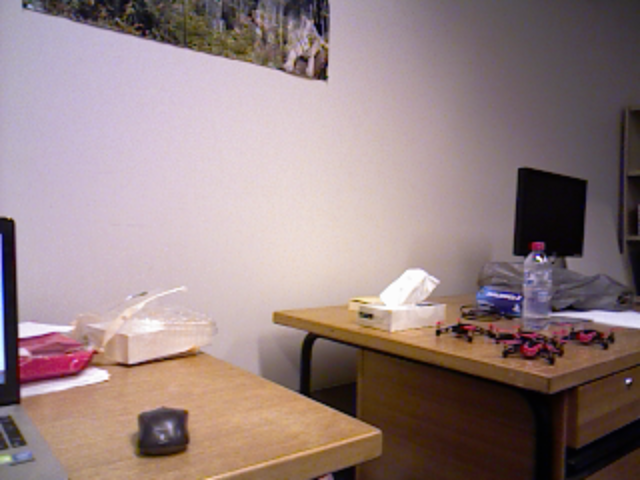
\includegraphics[width=1.7in]{images/ch2/colorF11}
                \caption{Color Image}
                \label{fig:COLEXAMPLE}
        \end{subfigure}%
        \begin{subfigure}[b]{1.8in}
                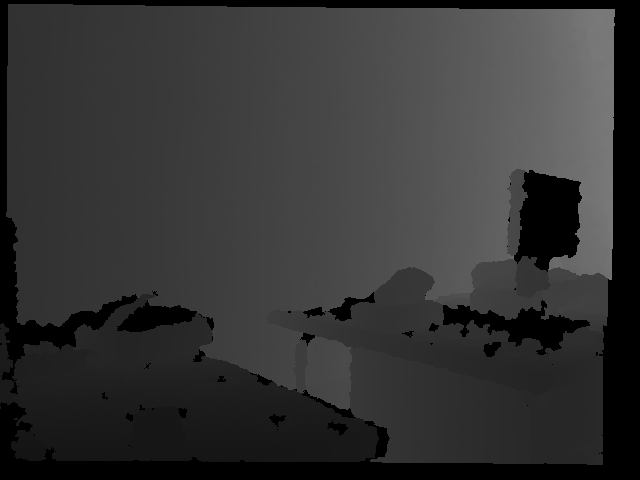
\includegraphics[width=1.7in]{images/ch2/depthF11}
                \caption{Depth Image}
                \label{fig:DEPTHEXAMPLE}
        \end{subfigure}
        
         \begin{subfigure}[b]{1.8in}
                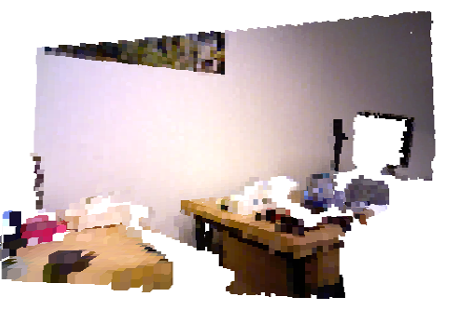
\includegraphics[width=1.8in]{images/ch2/volumeF11128}
                \caption{Projected Volume $128^3$}
                \label{fig:VOLUMEEXAMPLE128}
        \end{subfigure}%
         \begin{subfigure}[b]{1.8in}
                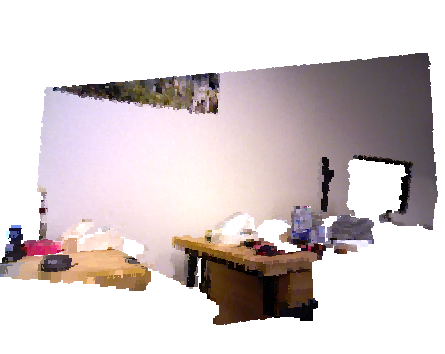
\includegraphics[width=1.8in]{images/ch2/volumeF11256}
                \caption{Projected Volume $256^3$}
                \label{fig:VOLUMEEXAMPLE384}
        \end{subfigure}%
       \caption{A Projected Frame.}
       \label{fig:PROJECTED_FRAME}
\end{figure}


To facilitate further processing, the projected image volumes are re-sampled. The results reported in this paper were obtained using volumes of $256^3$ voxels in size. An example colour and depth image pair and their volumetric projection is shown in figure \ref{fig:PROJECTED_FRAME}.  \\


\subsection{Stereo Camera Based Reconstruction}

The Fourier volume registration methods also work with stereo camera based data. This information can be generated using several of the techniques described in the literature review. Essentially the data must then be projected into depth frames which are registered using one of the proposed fourier volume registration techniques. Because stereo methods do not always accurately compute depth to scale, fourier volume registration has an advantage over other methods in that it also registers against scale. For systems where depth is estimated accurately (as accurately or more than depth sensors) results should work similarly.

\subsection{Monocular Sensor Based 3D Reconstruction}

Some preliminary research has been conducted in evaluating the use of Fourier volume registration given monocular data. From monocular video frames, depth was first computed. This data was fed into the fourier volume registration method in computing 3D reconstructions. Preliminary results are presented but further investigation is required in this area.



\section{Conclusion}